\documentclass[10pt, letterpaper]{article}
\usepackage[letterpaper,margin=1in]{geometry}
\usepackage{caption}
\usepackage{float}
\usepackage{amsmath}
\usepackage{amsfonts}
\usepackage{xspace}
\usepackage{titling}
\usepackage{graphicx}
\usepackage{subcaption}
\usepackage{todonotes}
% Authors and Title {{{
\author{Gillian Queisser (PI), Stephan Grein, James Rosado}
\title{\vspace{-2cm}Progress Report}
\date{\vspace{-1cm}}
% }}}

\begin{document}

\maketitle

\subsection*{Synaptic Spine Calcium Dynamics}
We would like to note that the manuscript \textit{Calcium modeling of spine apparatus containing human dendritic spines demonstrates all-or-nothing communication switch between the spine head and dendrite} which was supported by the current funding period has been submitted to a peer-reviewed journal and in this manuscript we state and explain the results summarized in this progress report.

The system of diffusion equations \cite{Breit2018} for modeling calcium dynamics is given by:
\begin{align}
    \frac{\partial c_c}{\partial t} &= D_c\Delta c_c + (\kappa_b^-(b^{tot}-b)-\kappa_b^+bc_c),\\
    \frac{\partial b}{\partial t} &= D_b\Delta b + (\kappa_b^-(b^{tot}-b)-\kappa_b^+bc_c),\\
    \frac{\partial c_e}{\partial t} &= D_c\Delta c_e, 
\end{align}
where $c_c$ is the cytosolic calcium and $c_e$ is calcium in the ER, $(b^{tot})$ is the total concentration of CalB present in the cytosol, and $\kappa_b^+$, $\kappa_b^-$ are rate constants. We also take into account influxes at the PSD, calcium exchange mechanisms located on the ER membrane and PM, the complete set of equations is described in (cite Breit,Queisser Paper). We first established a baseline for the level of calcium concentration in the cytosol when there is no ER inside the cytosol region of the geometry. The baseline simulations were executed using the 9 spine-dendrite geometries,  Figure \ref{fig:prg1}, row A, with no endoplasmic reticular (ER) and with passive ER, and a calcium influx was specified at the PSD for each spine. Both sets of baseline simulations revealed that passive/absent spine apparatus organelles (the ER) have no major impact on spine-to-dendrite calcium signaling. In all cases less than 3\%  of the initial calcium concentration amplitude in the head was detectable in the dendrite. When the ER was added as a passive compartment (i.e., when it was present as a geometric obstacle, but without any calcium exchange mechanisms), similar and near-zero dendritic calcium concentration profiles are observed in the respective spines Figure \ref{fig:prg1}, row B. Therefore, calcium influx at the PSD alone without intracellular calcium dynamics from the ER is not enough to induce spine-to-dendrite calcium coupling; in particular, only a small fraction of released $\textrm{Ca}^{2+}$ ions reaches the dendritic compartment. However, with active ER there exists a critical RyR density where by we have significant calcium signaling in the dendritic region Figure \ref{fig:prg1}, row C.

%\begin{figure}[h!]
%\centering
%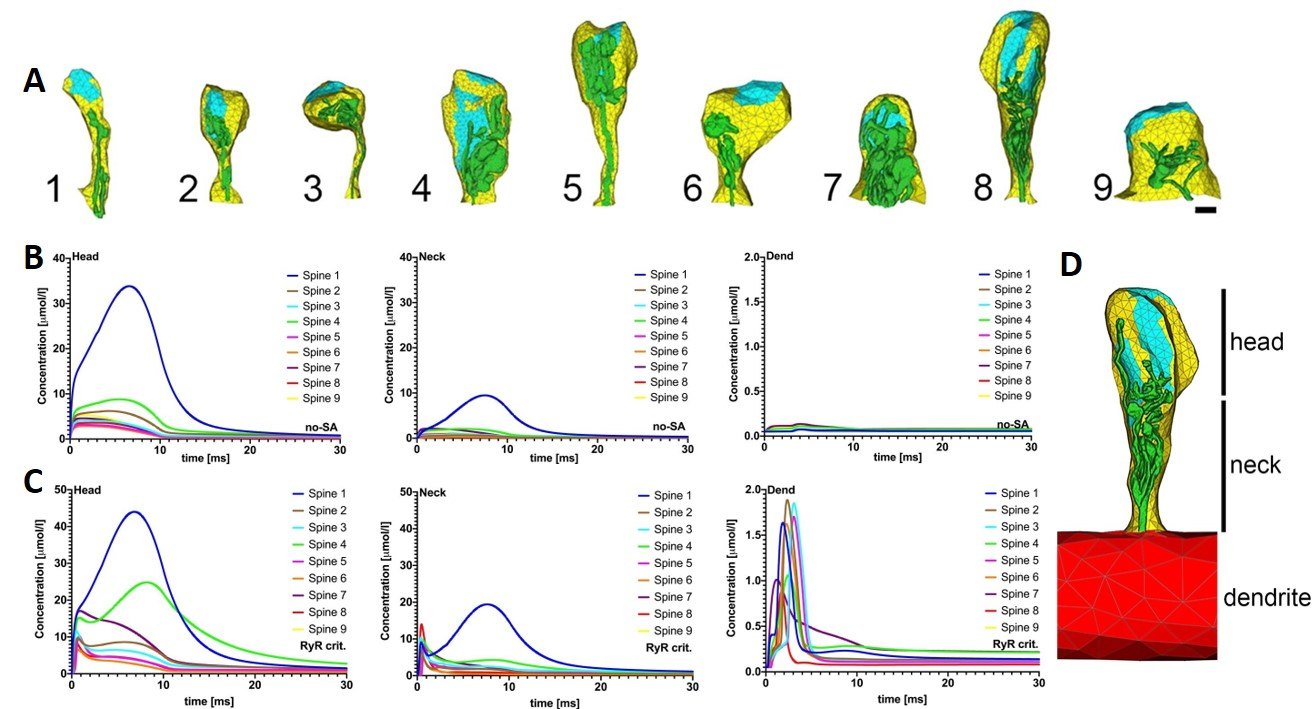
\includegraphics[width=0.5\linewidth]{img/Picture1.jpg}
%\caption{}
%\label{fig:prg1}
%\end{figure}

\begin{figure}
     \centering
     \begin{subfigure}[b]{0.45\textwidth}
         \centering
         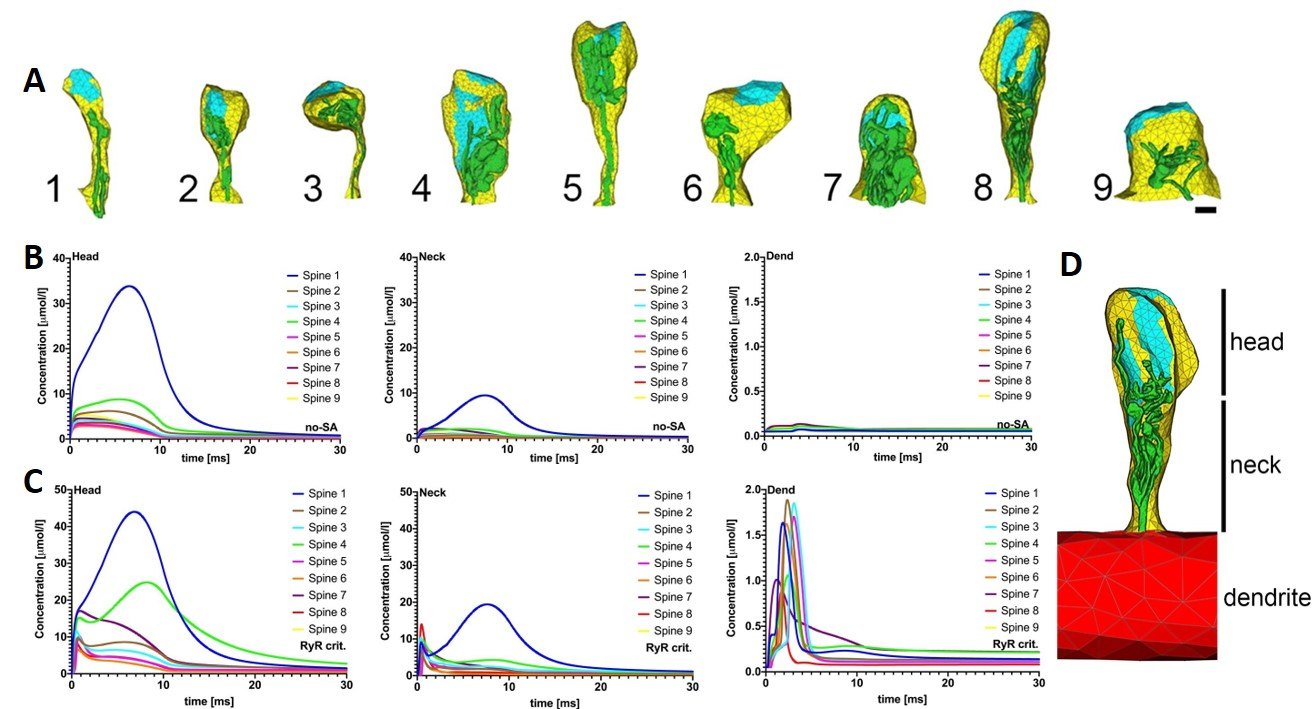
\includegraphics[width=\textwidth]{img/Picture1.jpg}
         \caption{}
         \label{fig:prg1}
     \end{subfigure}
     \begin{subfigure}[b]{0.45\textwidth}
         \centering
         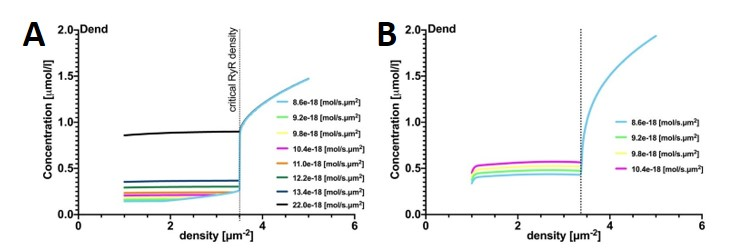
\includegraphics[width=\textwidth]{img/Picture2.jpg}
	\caption{}
         \label{fig:prg2}
     \end{subfigure}
\caption{In (a) we show the types of spine geometries and the calcium profiles. (b) shows a vertical \textit{jump} in the concentration of the dendritic cytosol. (b) demonstrates that the critical RyR density is invariant under changes in synaptic calcium influx and calcium buffering. Figure (b)-A is full buffering of calcium and Figure (b)-B  is half buffering of calcium.}
\end{figure}

We determined that when the ER is active with RyRs and SERCA pumps there is a critical RyR density $\rho_{RyRcrit}$, Figure \ref{fig:prg2}-A, such that if $\rho_{RyR}<\rho_{RyRcrit}$ then there is no spine-dendrite calcium signaling and if $\rho_{RyR}\geq\rho_{RyRcrit}$ there is spine-to-dendrite calcium signaling. This was carried out by running a sequence of simulations where the RyR density parameters was increased  starting from 0.00 $\mu m^{-2}$ to 5.00 $\mu m^{-2}$ at increments of 0.01 $\mu m^{-2}$. We tested whether changes in $\textrm{Ca}^{2+}$ entry at the synapse affect the critical RyR density by successively increasing the $\textrm{Ca}^{2+}$ flux density at the PSD, changes in the level of calcium buffering present in the cytosol (Figure \ref{fig:prg2}-A is full buffering, Figure \ref{fig:prg2}-B is half buffering) and the simulations demonstrate that calcium coupling occurs at the same RyR density, regardless of the initial $\textrm{Ca}^{2+}$ influx and changes in calcium buffering, Figure \ref{fig:prg2}-B. Therefore, ryanodine receptors of spine apparatus control spine-to-dendrite $\textrm{Ca}^{2+}$ signaling. We also carried out simulations by which we varied the neck diameter of the spine morphologies, and we observed a positive correlation between spine and SA cross-sectional area of the spine neck. This suggests that the ER adjusts to dendritic spine growth and reorganizes in such a way to support spine-to-dendrite $\textrm{Ca}^{2+}$ communication. In fact, previous work has demonstrated that changes in spine neck diameters accompany the induction of excitatory synaptic plasticity, reflected by an increase in spine head size \cite{Araya2014,Tonnesen2014,Steffens2021}. Simulations are ongoing and below in Table 1 we have listed our current usage (as of submission of the renewal request) and tentative usage for the remaining 20\% of project duration.

% Please add the following required packages to your document preamble:
% \usepackage{graphicx}
\begin{table}[h!]
\centering
\resizebox{0.3\textwidth}{!}{%
\begin{tabular}{|c|l|l|l|}
\hline
\multicolumn{2}{|c|}{\textbf{\begin{tabular}[c]{@{}c@{}}Synaptic Spine   \\ Calcium Dynamics\end{tabular}}} & \multicolumn{2}{c|}{\textbf{\begin{tabular}[c]{@{}c@{}}Full Cell Calcium\\ Dynamics\end{tabular}}} \\ \hline
\textbf{Simulation} & \multicolumn{1}{c|}{\textbf{SU}} & \multicolumn{1}{c|}{\textbf{Simulation}} & \multicolumn{1}{c|}{\textbf{SU}} \\ \hline
\multicolumn{1}{|r|}{Baseline Runs} & 13,188 & Synaptic strength Runs & 128,052 \\ \hline
\multicolumn{1}{|r|}{RyR Runs} & 20,300 & Synapse loss Runs & 13,426 \\ \hline
\multicolumn{1}{|r|}{Pulse Runs} & 12,706 & Stimulation Region Runs & 28,196 \\ \hline
\multicolumn{1}{|r|}{VDCC Runs} & 207,710 &  &  \\ \hline\hline
\multicolumn{4}{|c|}{\textbf{Tentative Usage}} \\ \hline
\textbf{Simulation} & \multicolumn{1}{c|}{\textbf{SU}} & \multicolumn{1}{c|}{\textbf{Simulation}} & \multicolumn{1}{c|}{\textbf{SU}} \\ \hline
\multicolumn{1}{|l|}{Pulse Runs} & 100,000 & Synapse Loss & 120,000 \\ \hline
\multicolumn{1}{|l|}{VDCC Runs} & 80,000 & Stimulation Regions & 120,000 \\ \hline
\end{tabular}%
}
\caption{SU usage according to project simulations.}
\label{tab:sus}
\end{table}

We are currently running simulations, \texttt{TMS runs}, incorporating voltage dependent calcium channels (VDCCs) to determine under what conditions we have strong spine-to-dendrite calcium signalling and calcium wave propagation through the dendrite. Current simulation results demonstrate that having either PSD calcium influx or VDCC  release is sufficient for calcium signaling to the dendrite; however, having each alone is not enough to produce stable calcium wave propagation.

%\begin{figure}[h!]
%\centering
%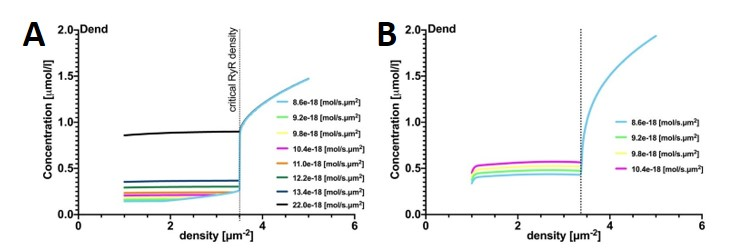
\includegraphics[width=0.45\linewidth]{img/Picture2.jpg}
%\caption{Figure A shows a vertical \textit{jump} in the concentration of the %dendritic cytosol. Figure B demonstrates that the critical RyR density is %invariant under changes in synaptic calcium influx and calcium buffering. %Figure A is full buffering of calcium and Figure B is half buffering of %calcium.}
%\label{fig:prg2}
%\end{figure}

\subsection*{Whole Cell Dynamics Progress}
For the subproject \textbf{Whole Cell Dynamics} under investigation, the authors
would like to note that two manuscript are currently in preparation resulting from a 
recently completed PhD dissertation \cite{Grein2020} and supported by simulations on the XSEDE
SDSC Comet cluster discussing the meshing pipeline and neurobiological implications
of intracellular calcium waves - an excerpt of the results to be published will be
given in the report below.

To determine a threshold for the number of synapses required to generate stable 
intracellular calcium waves as a communication device from distal (neurite tips) 
to proximal regions (soma) a parameter variation of synaptic activation strength
was conducted as proposed in the original allocation request, see Tab. \ref{tab:sus}.
Specifically, a variation of synaptic activation strength has been conducted, in which
the low and high synaptic strength has been used for the activation of synapses.
While strong synapses reliably trigger intracellular calcium waves, we determined
a threshold for the number of weak synapses with a fully synchronous activation
pattern as depicted in Fig. \ref{fig:wave} and proposed previously. Based on this
calibration, synapse loss studies are currently being conducted on 6 representative 
cells, as well as well as a comparison of 10 morphologically distinct neurons,
to investigate the effects of a variation of spatial stimulation as presented in
the proposal. For this, the remaining budget of the current allocation
will be used (see Tab.~\ref{tab:sus} for a summary of the estimated number of
SUs in the remaining compute period).

\begin{figure}[h!]
\centering
\begin{subfigure}{.3\linewidth}
    \centering
    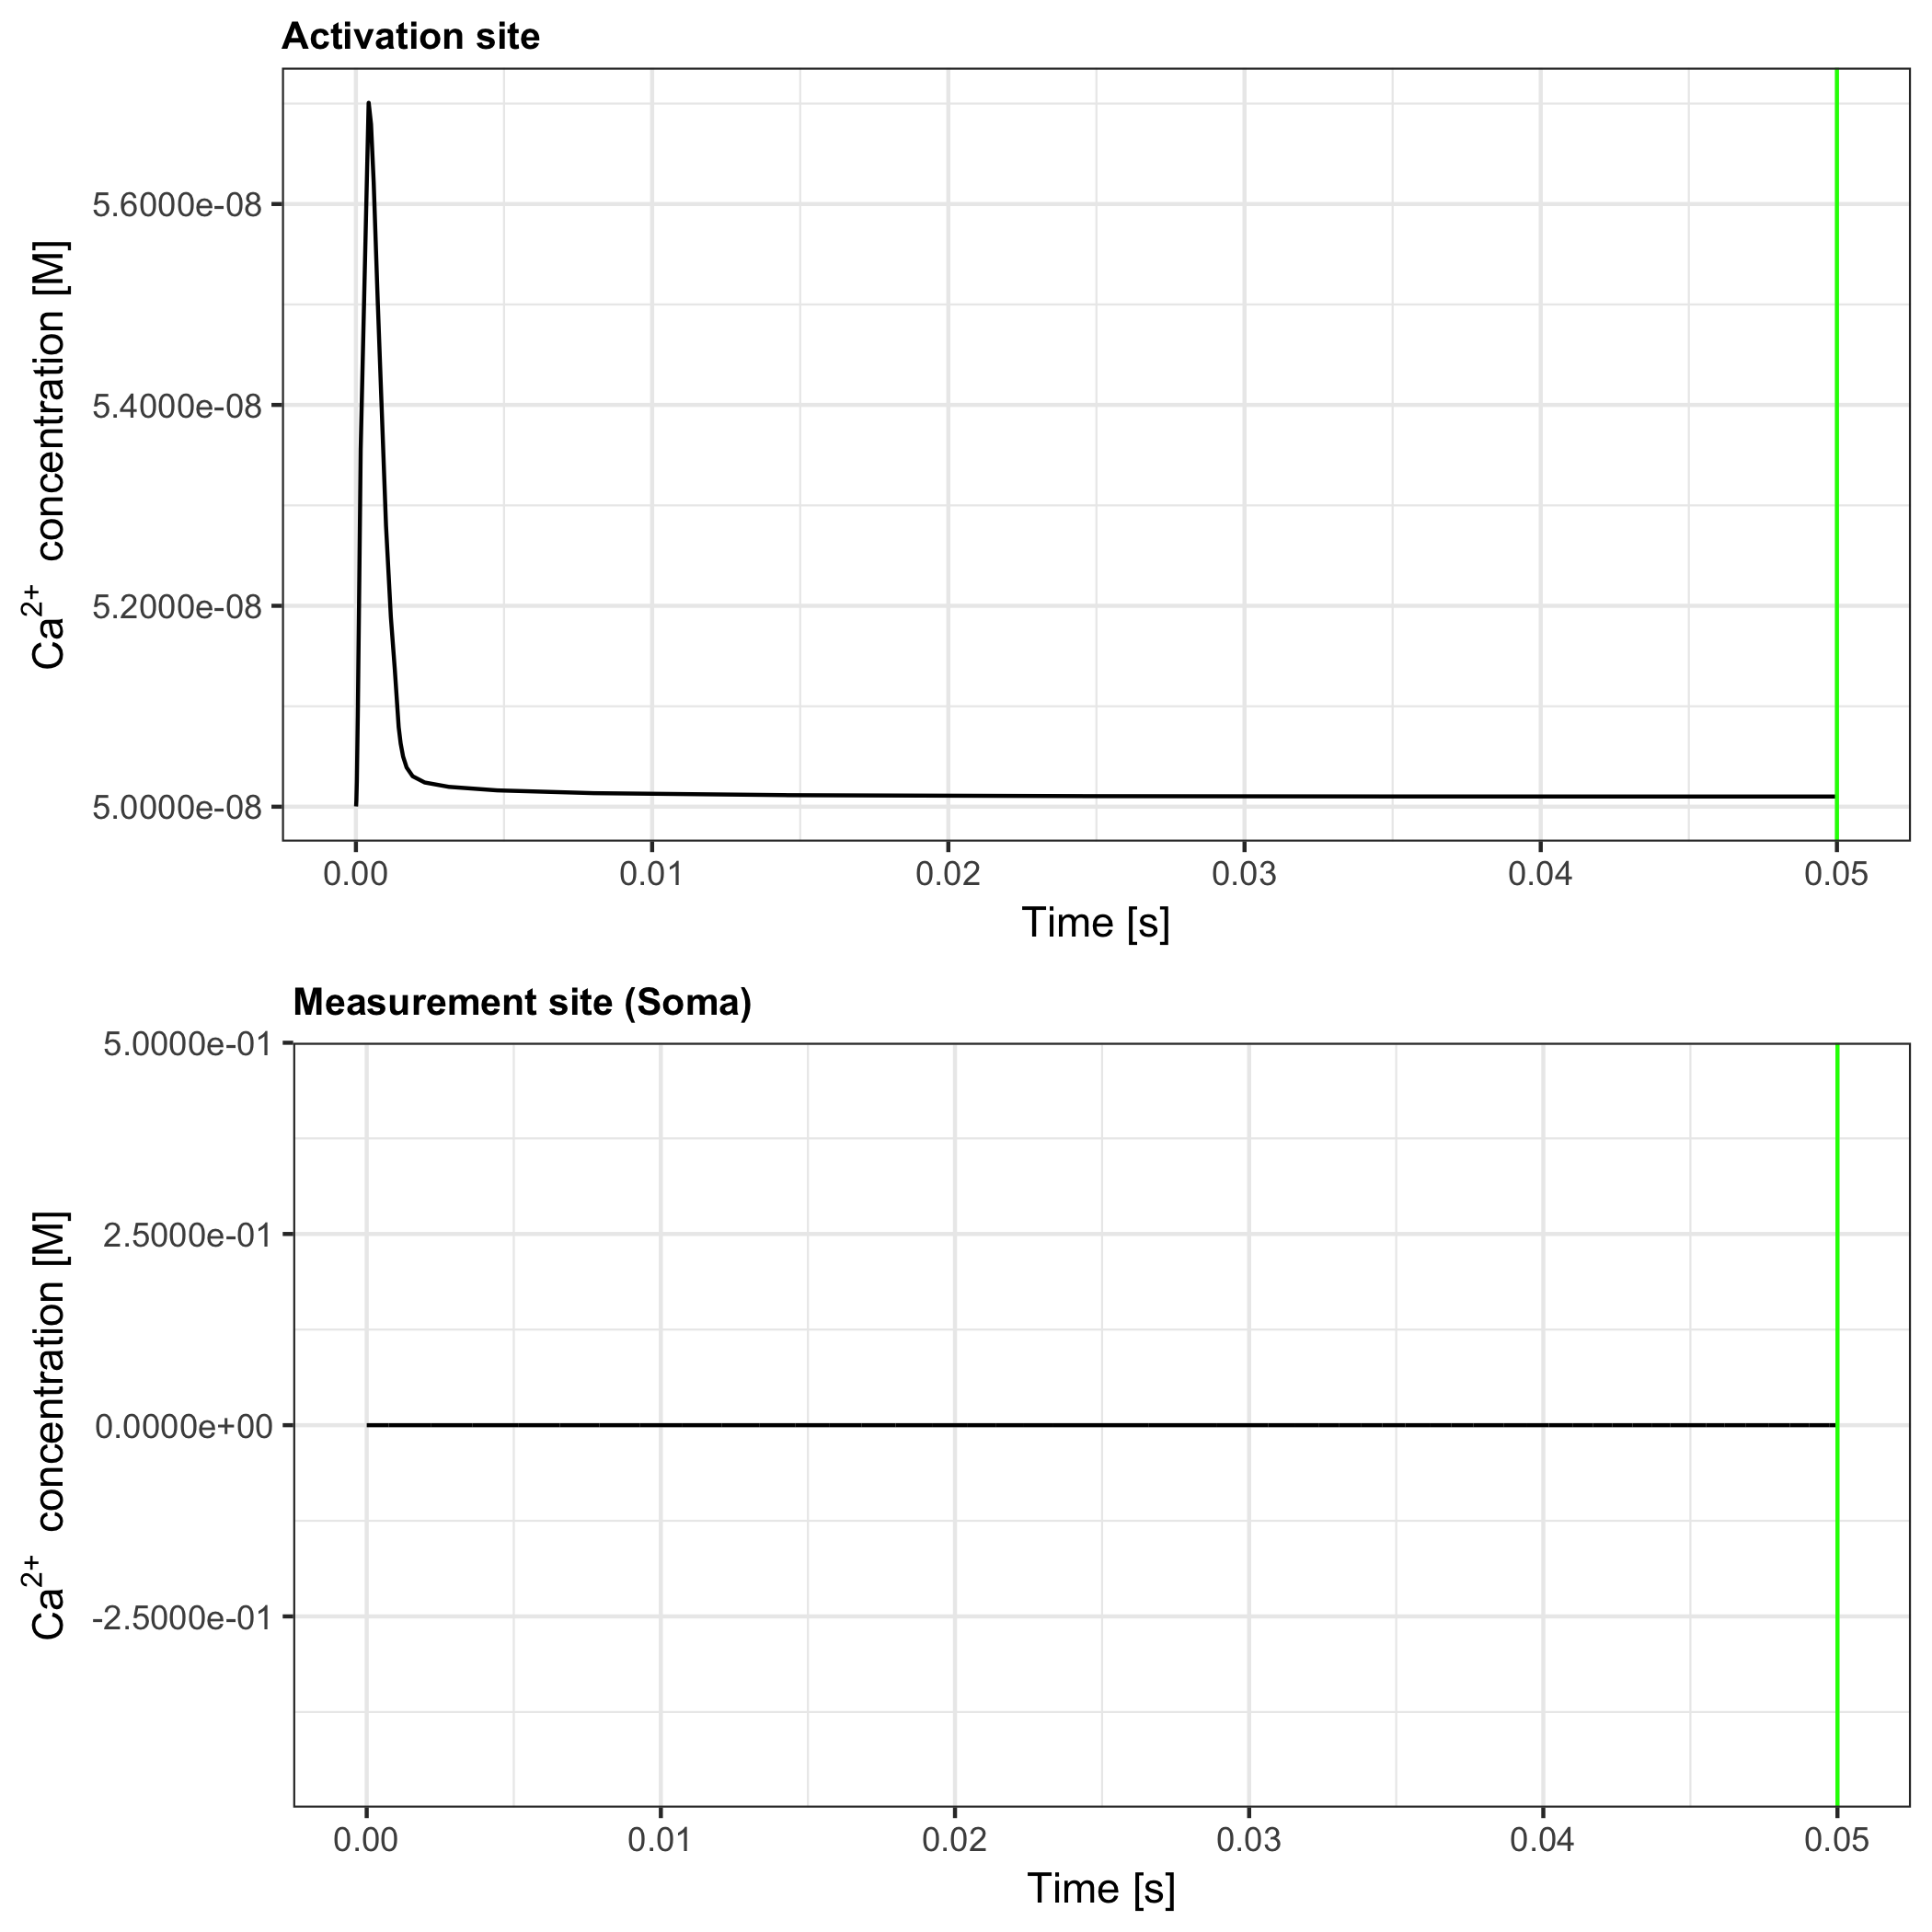
\includegraphics[scale=0.05]{img/example1.png}  
    \caption{$n=1$ synapses}\label{fig:image1}
\end{subfigure}
    \hfill
\begin{subfigure}{.3\linewidth}
    \centering
    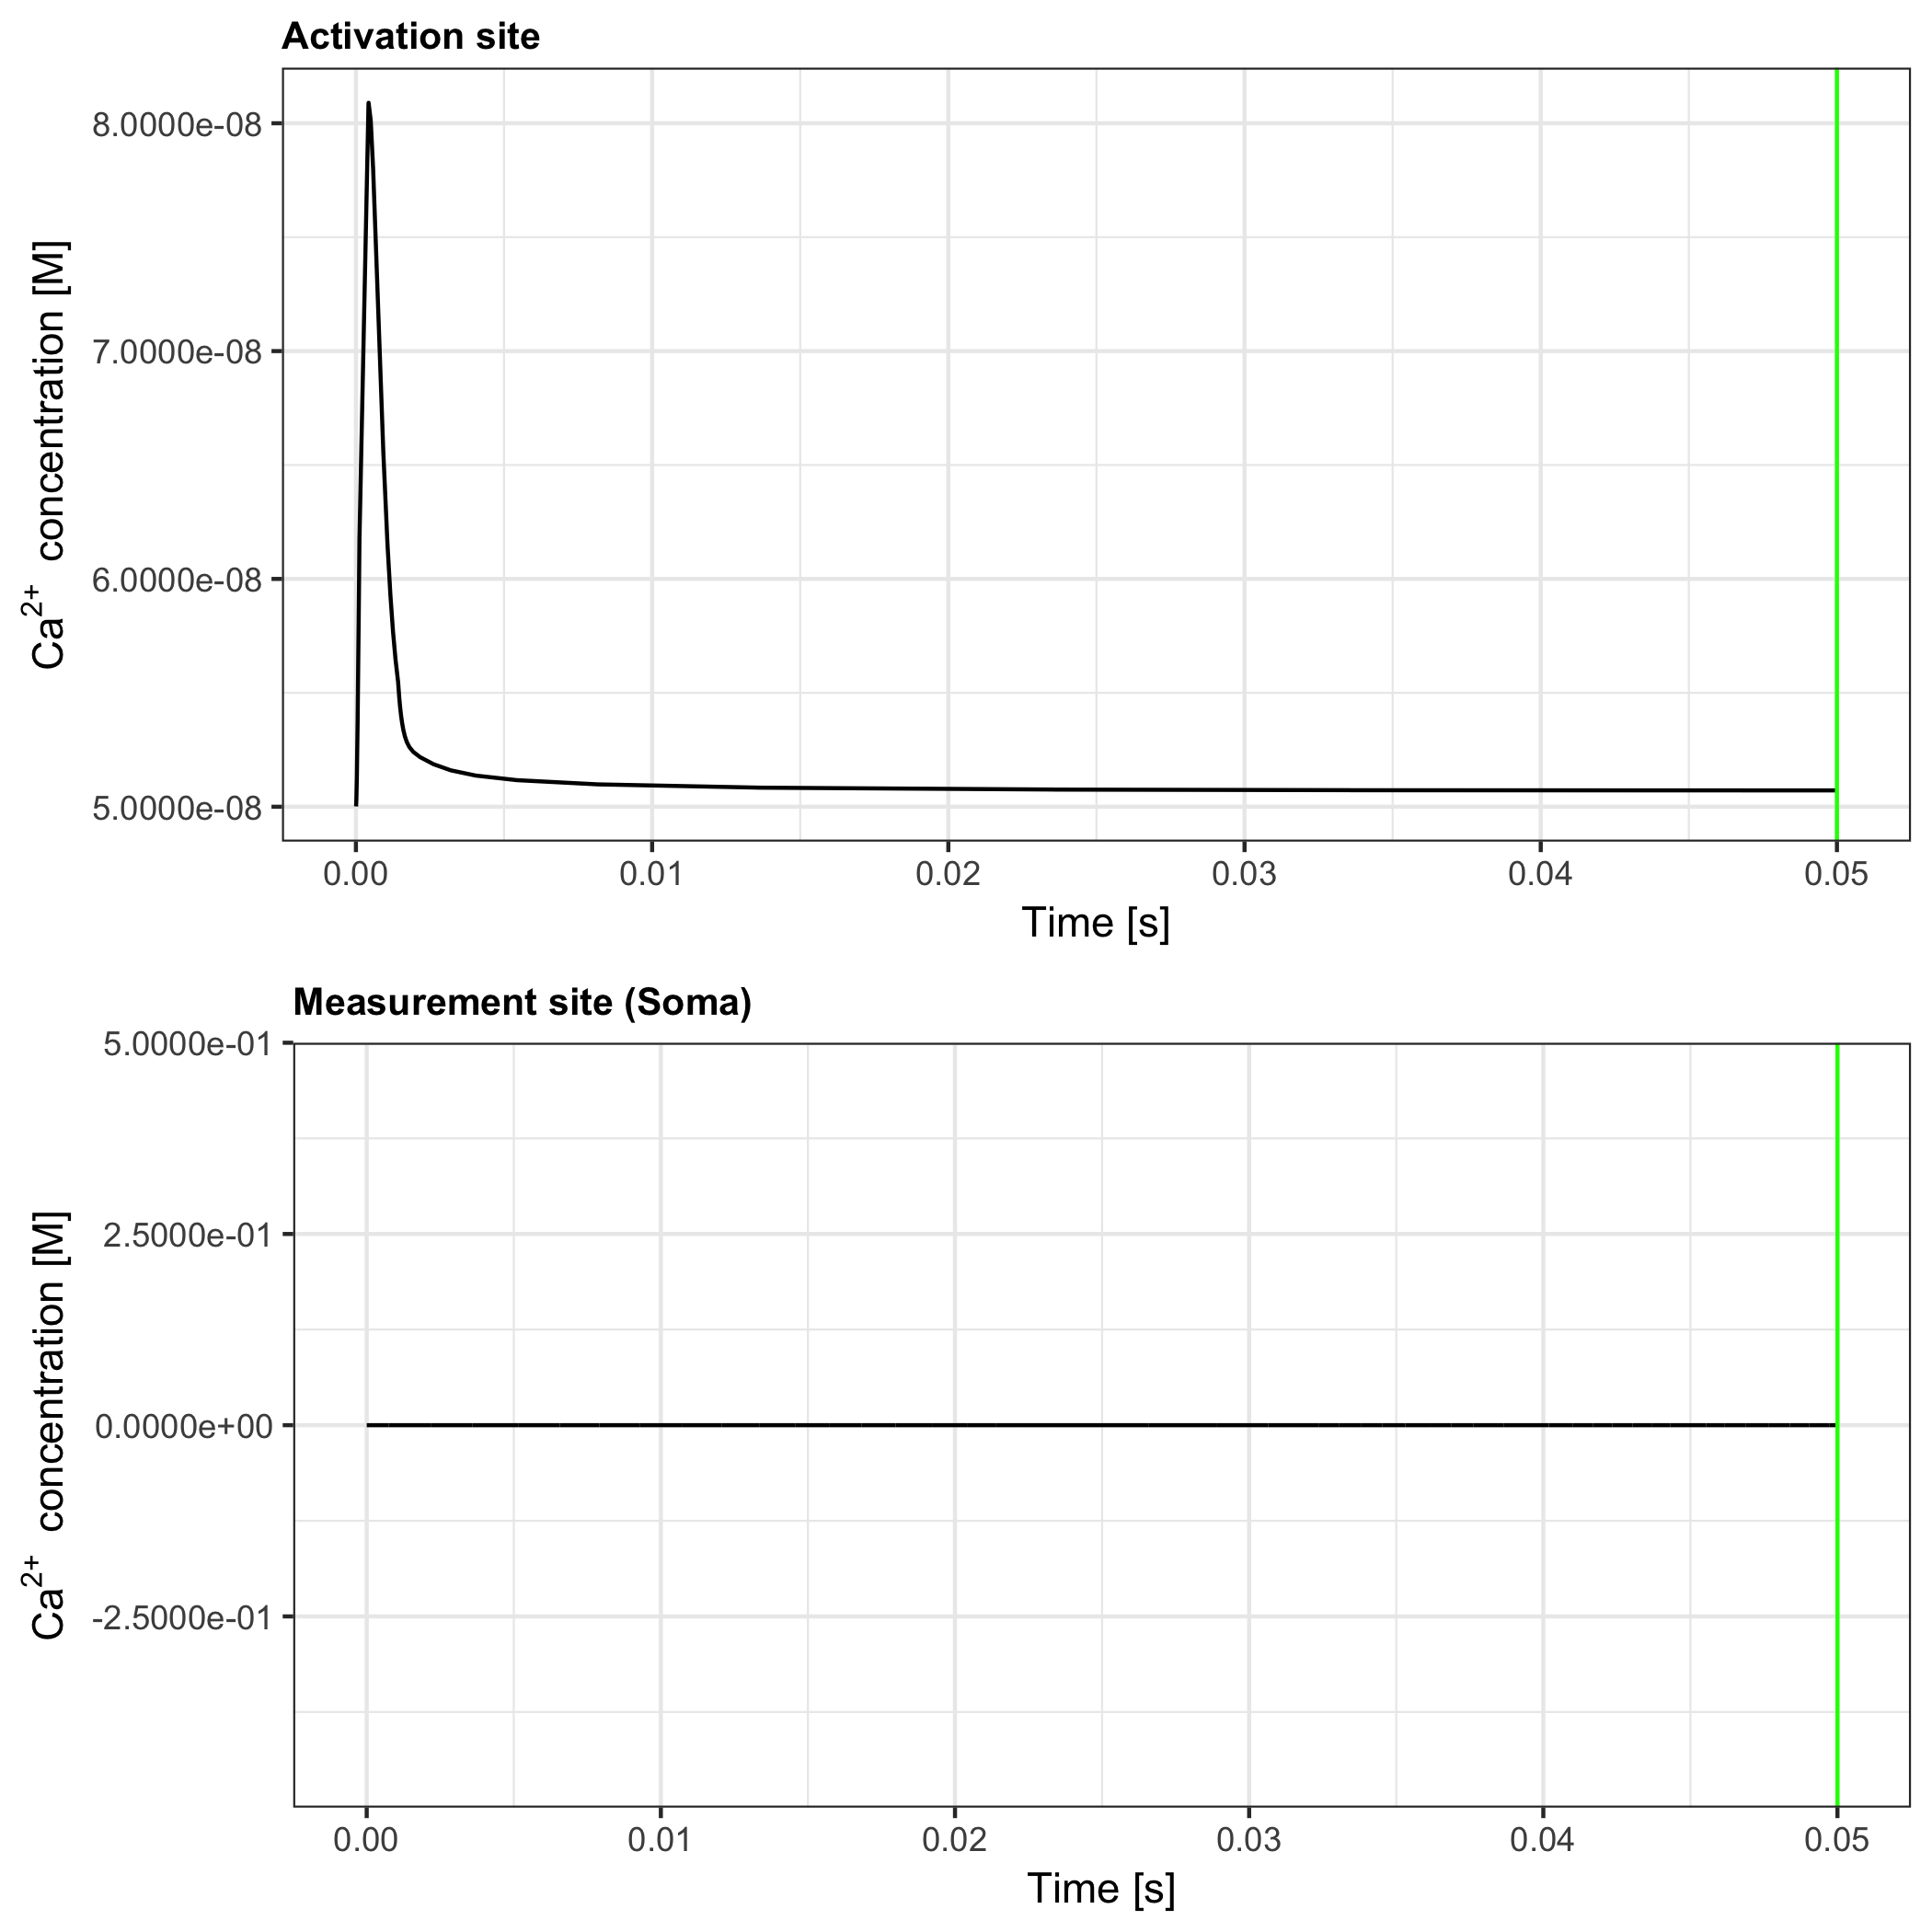
\includegraphics[scale=0.05]{img/example2.png}  
    \caption{$n=10$ synapses}\label{fig:image12}
\end{subfigure}
   \hfill
\begin{subfigure}{.3\linewidth}
    \centering
    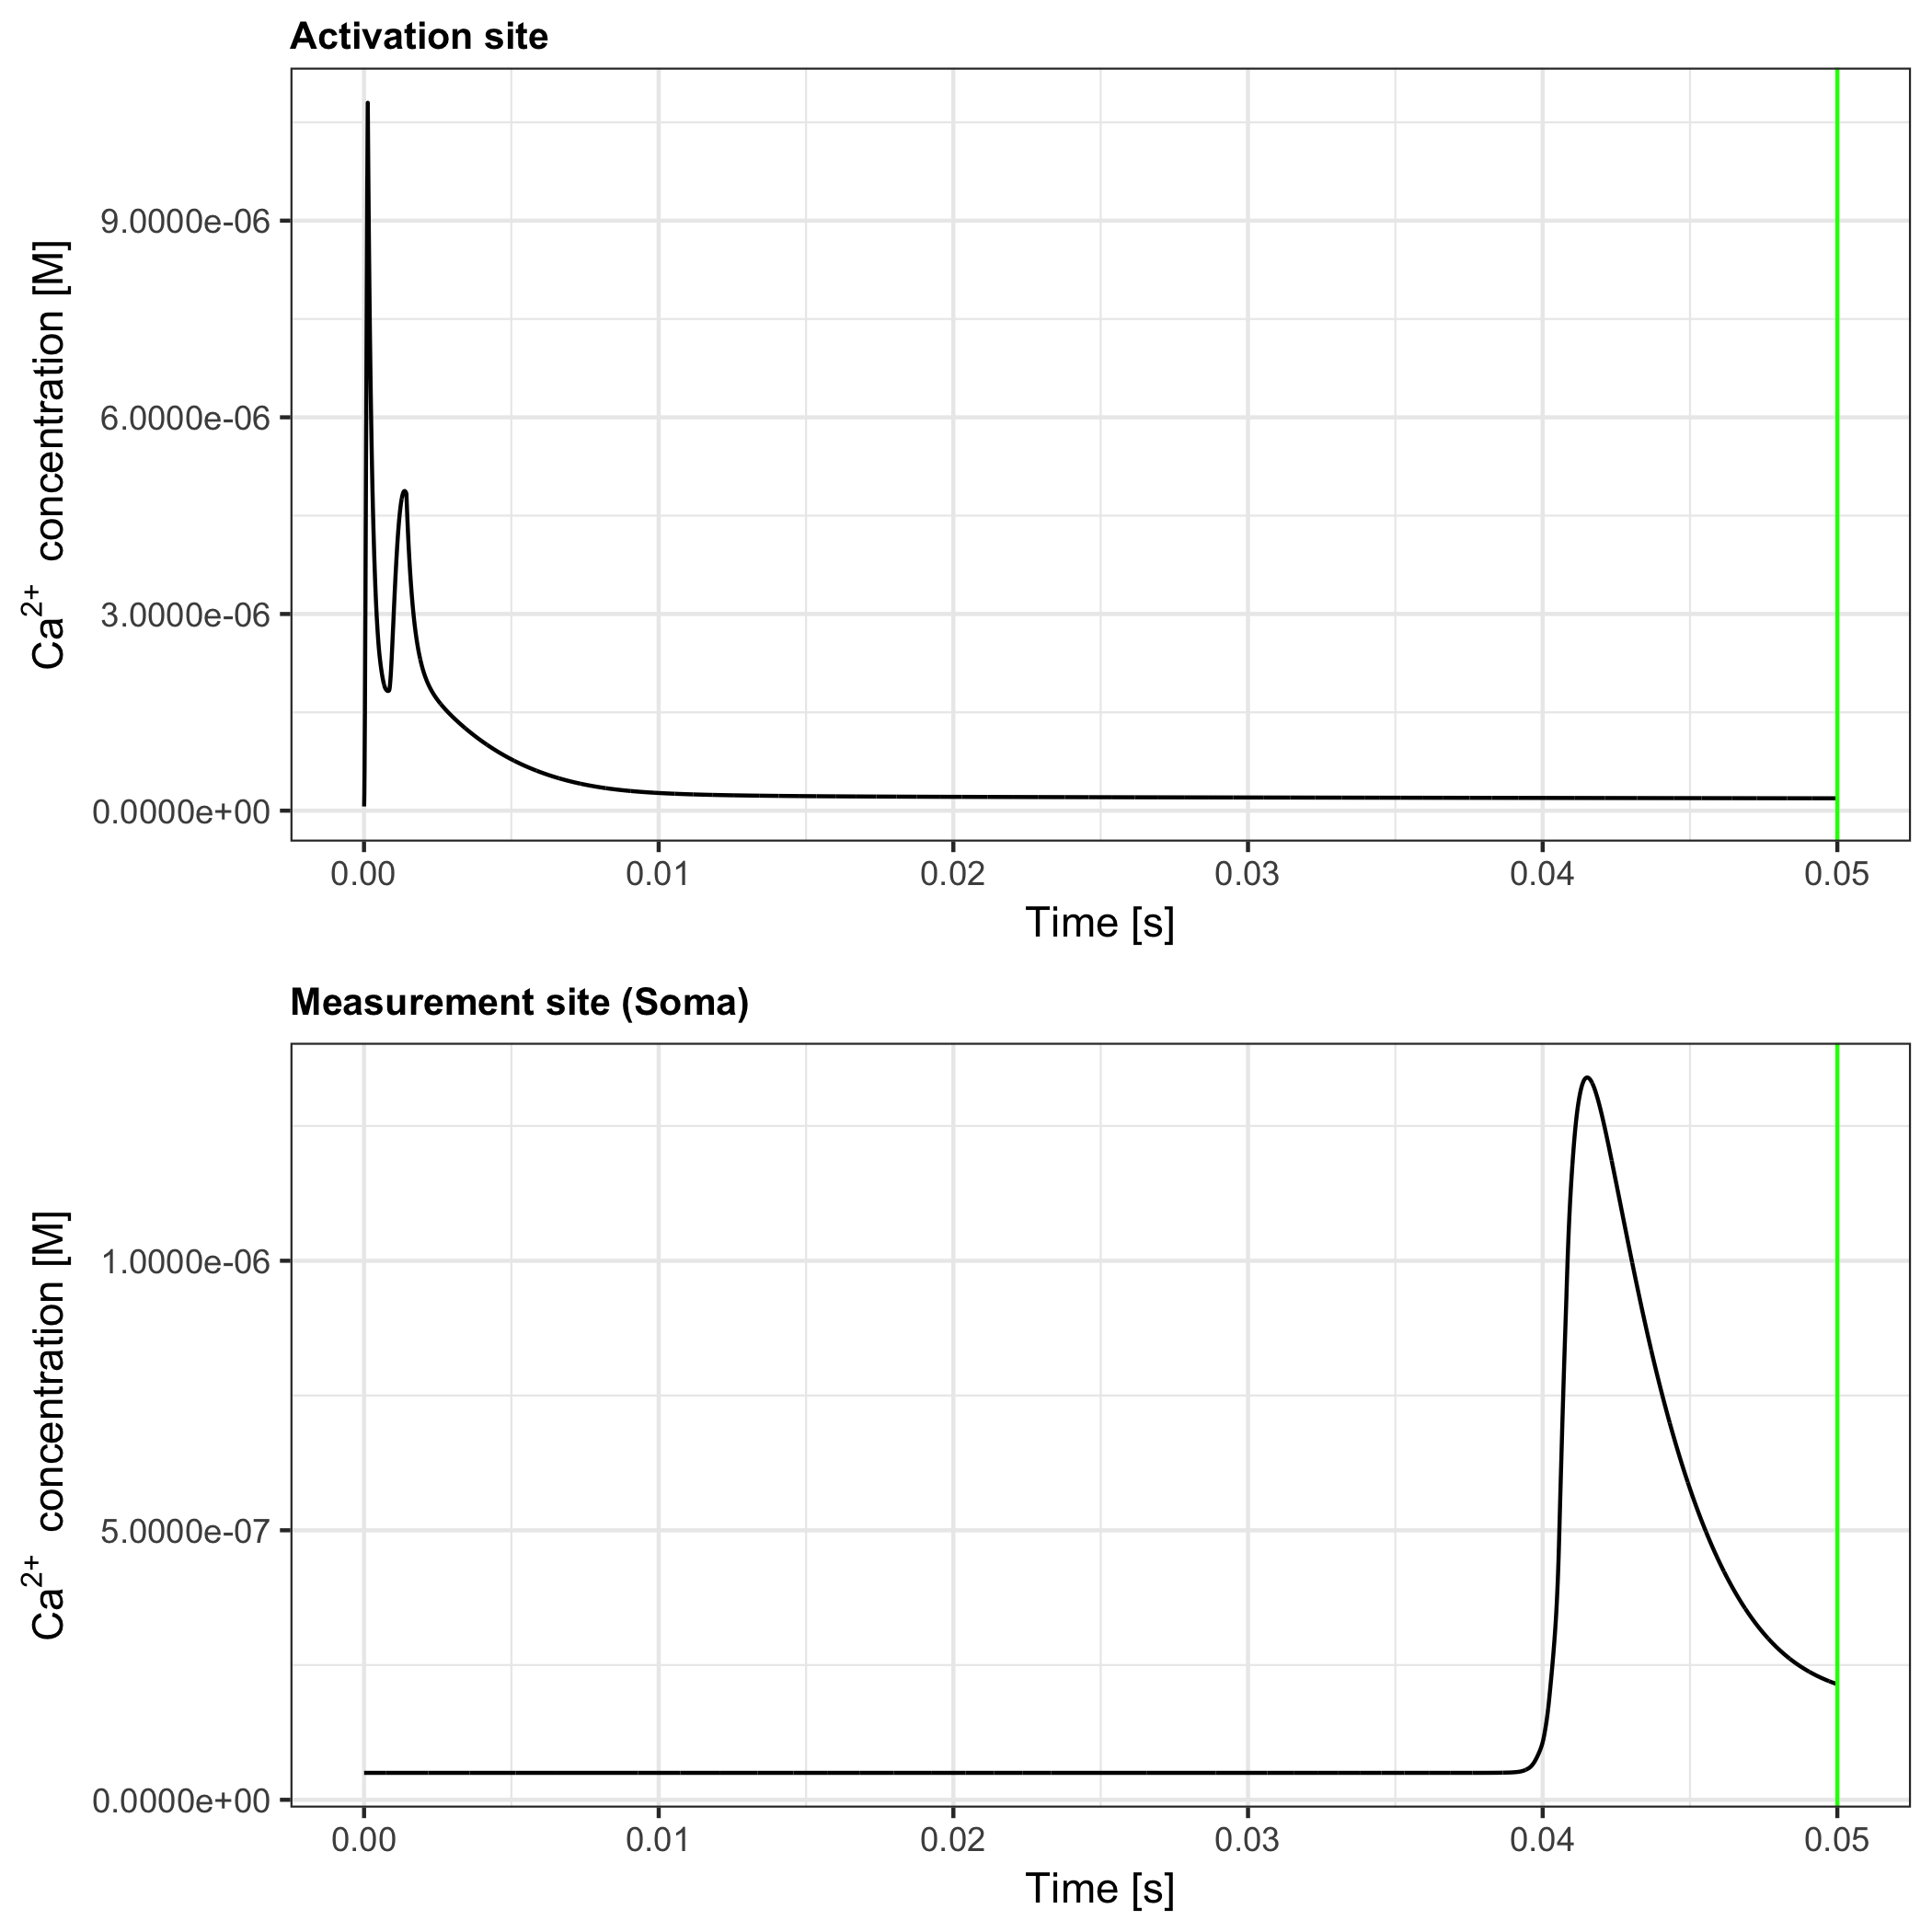
\includegraphics[scale=0.05]{img/example3.png}  
    \caption{$n=100$ synapses}\label{fig:image13}
\end{subfigure}
\caption{Synapse density threshold experiment: A stable intracellular calcium wave could be elicitated by 
stimulation of the input region (distal dendrites) with $n=100$ synapses on a cell from the Rice-Baylor
archive (entorhinal cortex). Vertical green bar indicates end of simulation time (50 ms).}
\label{fig:wave}
\end{figure}

Preliminary studies on synaptic strength are being combined with synapse loss studies and a variation of stimulation 
regions on various neurons. For this the 
remaining budget of service units on SDSC Comet and Expanse will be used to enable and support the finalizing of the two manuscripts in preparation. 

\subsubsection*{Explanation for under utilization of research allocation}
In the original proposal, the Synaptic Spine calcium subproject requested 270,000 SUs for RyR runs, and 607,500 SUs for the Calcium pulse runs; however, we decreased the number of runs in order to accommodate the 800,000 SUs we were granted. Overall, the international consortium for TMS-research was slowed down, due to COVID-related restrictions on travel and joint in-person research.
%In particular, we scaled down the number of runs for RyR simulations as recommended by reviewer feedback of the proposal, but also we established a smaller range of RyR density values to run our RyR simulations through. 
We also observed that not all spine simulations required equal amounts of simulation wall-time, this is determined by the complexity of the Spine-ER geometry and the density of RyRs on the ER membrane. In order to study the full level of calcium dynamics in the cytosol, we incorporated the VDCC simulations (\texttt{TMS runs} referenced in the main document) prior to continuing our runs of Calcium Pulse simulations. We anticipate completing our study of the \texttt{TMS} simulation results first, which will use most of the remaining SUs. Once the \texttt{TMS} simulations are complete, then we will execute our Calcium Pulse simulations which we anticipate using a minimum of 100,000 SUs, either from the new allocation or use any remaining SUs. Likewise the Whole Cell Calcium Dynamics project used narly the 150,000 SUs which have been requested in the original proposal for a systematic evaluation of the consequences of synaptic strength on intracellular calcium waves and calcium signaling. During these studies it has been recognized that runtime for simulations can be reduced depending on the stimulation setup, thus less SUs had been required contrary to our expectation. Still the remaining 350,000 service units will be required to complete the tasks of systematic studies on synapse location on realistic cell geometries and synapse loss studies in this subproject. The available SUs will be manually load-balanced in the next two month between the subprojects depending on the priority of simulations for the progression of the projects' research, see tentative usage in Tab. \ref{tab:sus} above.

\bibliography{export}
 \bibliographystyle{plain}

\end{document}
